\begin{apendicesenv}

\chapter{Diagramas de Blocos da Rede Rural de Ibirama -- SC (PON Planner)}
\label{apendice:diagramas_ibirama}

Este apêndice apresenta os diagramas de blocos detalhados da topologia óptica rural de Ibirama -- SC desenvolvida no \textit{PON Planner} (Teste 2), divididos em três seções sequenciais para garantir a legibilidade visual de todos os nós, enlaces e parâmetros técnicos.

\section{Topologia Desbalanceada Inicial (Com Nós Inoperantes em Vermelho)}

As Figuras~\ref{fig:ap_desbal_b1}, \ref{fig:ap_desbal_b2} e \ref{fig:ap_desbal_b3} ilustram os três blocos da rede rural desbalanceada no \textit{PON Planner}, destacando as atenuações excessivas nas últimas CTOs.

\begin{figure}[htb]
    \caption{Bloco 1 (Inicial) da topologia desbalanceada no \textit{PON Planner} -- OLT, CEO e CTOs 01 a 05}
    \label{fig:ap_desbal_b1}
    \centering
    \parbox{16cm}{
        \centering
        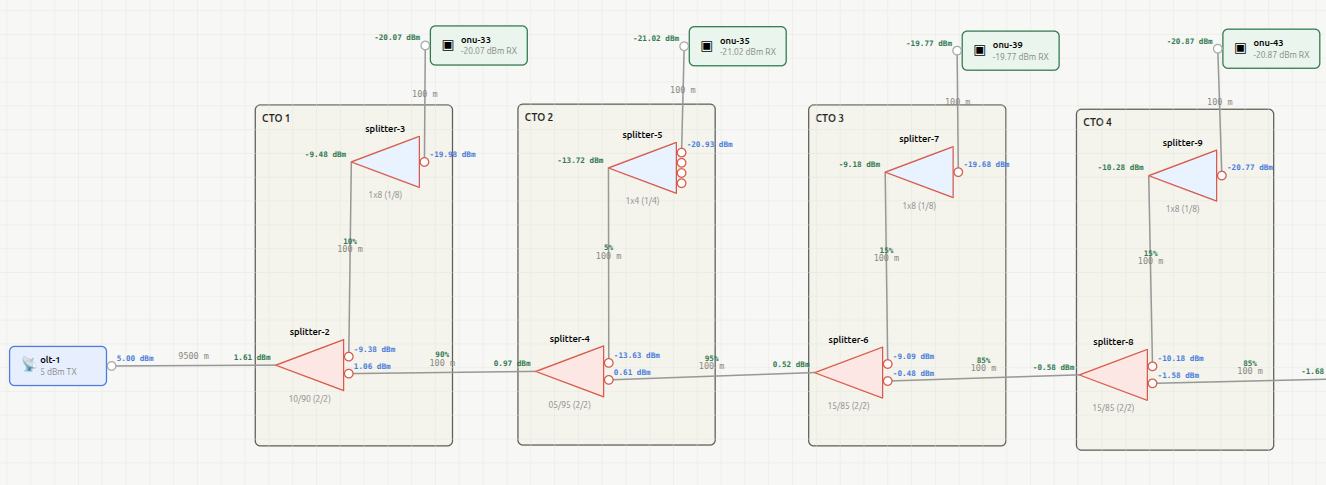
\includegraphics[width=0.95\textwidth]{images/ponplanner_ibirama_desbal_bloco1.png}
        \par\footnotesize Fonte: Tela capturada da aplicação \textit{PON Planner}.
    }
\end{figure}

\begin{figure}[htb]
    \caption{Bloco 2 (Intermediário) da topologia desbalanceada no \textit{PON Planner} -- CTOs 06 a 10}
    \label{fig:ap_desbal_b2}
    \centering
    \parbox{16cm}{
        \centering
        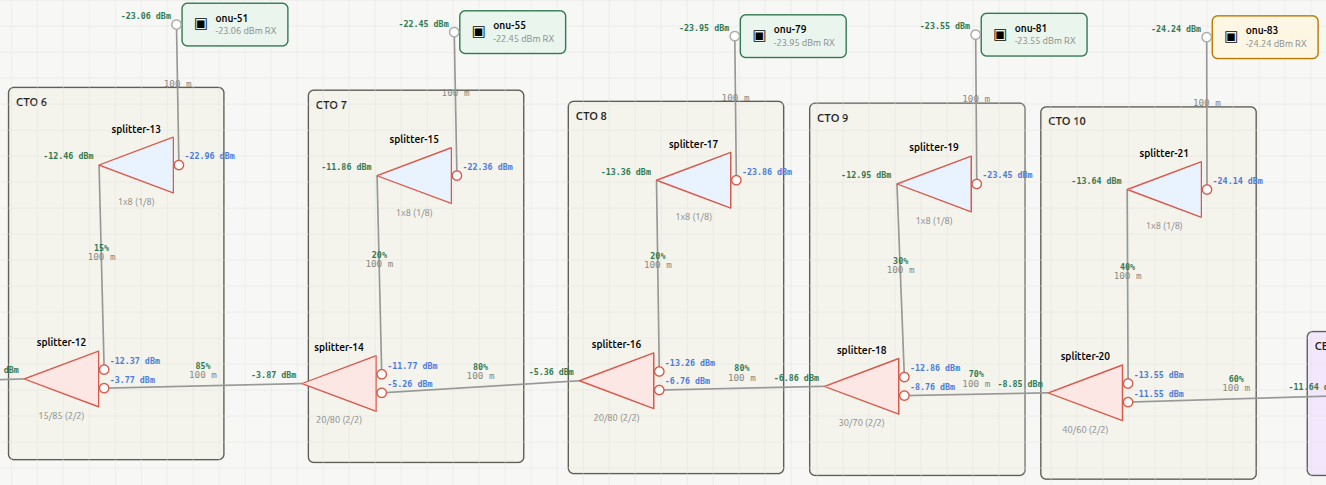
\includegraphics[width=0.95\textwidth]{images/ponplanner_ibirama_desbal_bloco2.png}
        \par\footnotesize Fonte: Tela capturada da aplicação \textit{PON Planner}.
    }
\end{figure}

\begin{figure}[htb]
    \caption{Bloco 3 (Final) da topologia desbalanceada no \textit{PON Planner} -- CTOs 11 a 14 com nós inoperantes}
    \label{fig:ap_desbal_b3}
    \centering
    \parbox{16cm}{
        \centering
        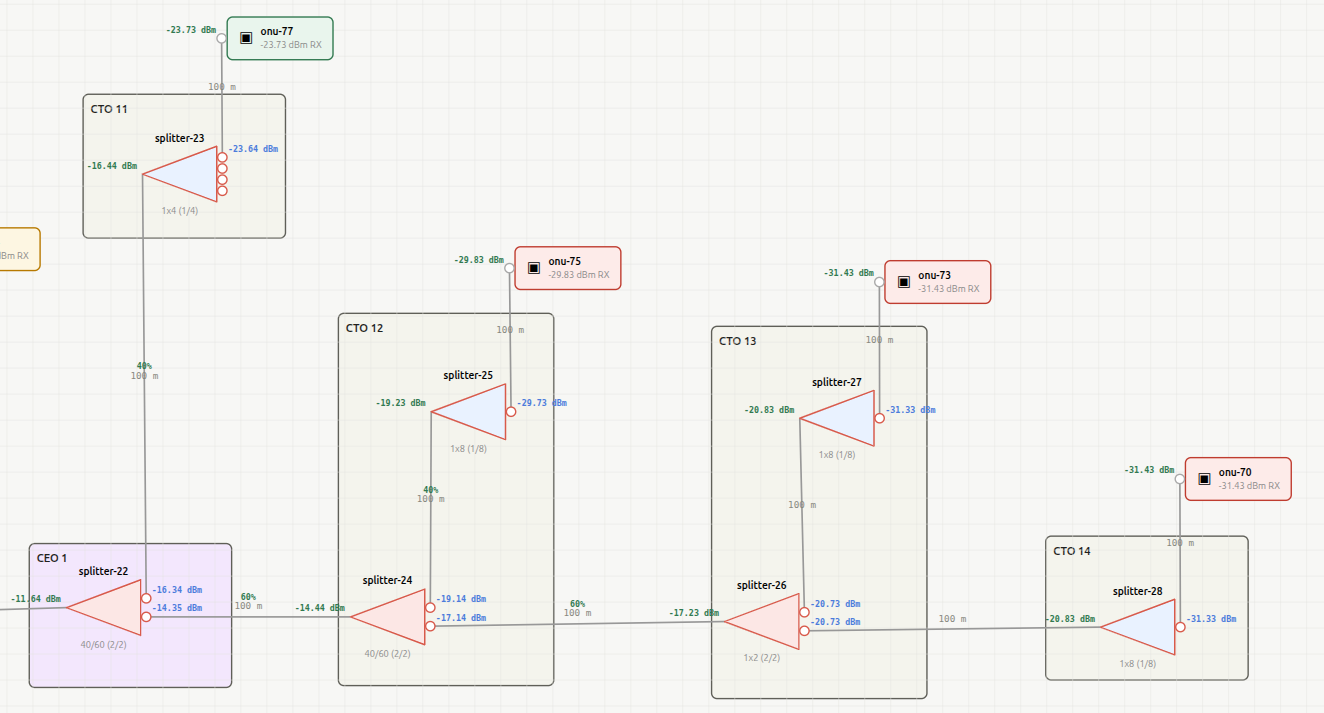
\includegraphics[width=0.95\textwidth]{images/ponplanner_ibirama_desbal_bloco3.png}
        \par\footnotesize Fonte: Tela capturada da aplicação \textit{PON Planner}.
    }
\end{figure}

\cleardoublepage

\section{Topologia Otimizada e Balanceada (Nós Operacionais em Verde)}

As Figuras~\ref{fig:ap_bal_b1}, \ref{fig:ap_bal_b2} e \ref{fig:ap_bal_b3} ilustram os três blocos da rede rural após a equalização completa dos \textit{splitters} desbalanceados no \textit{PON Planner}, com todos os ramais em faixa operacional verde.

\begin{figure}[htb]
    \caption{Bloco 1 (Inicial) da topologia balanceada no \textit{PON Planner} -- CTOs 01 a 05}
    \label{fig:ap_bal_b1}
    \centering
    \parbox{16cm}{
        \centering
        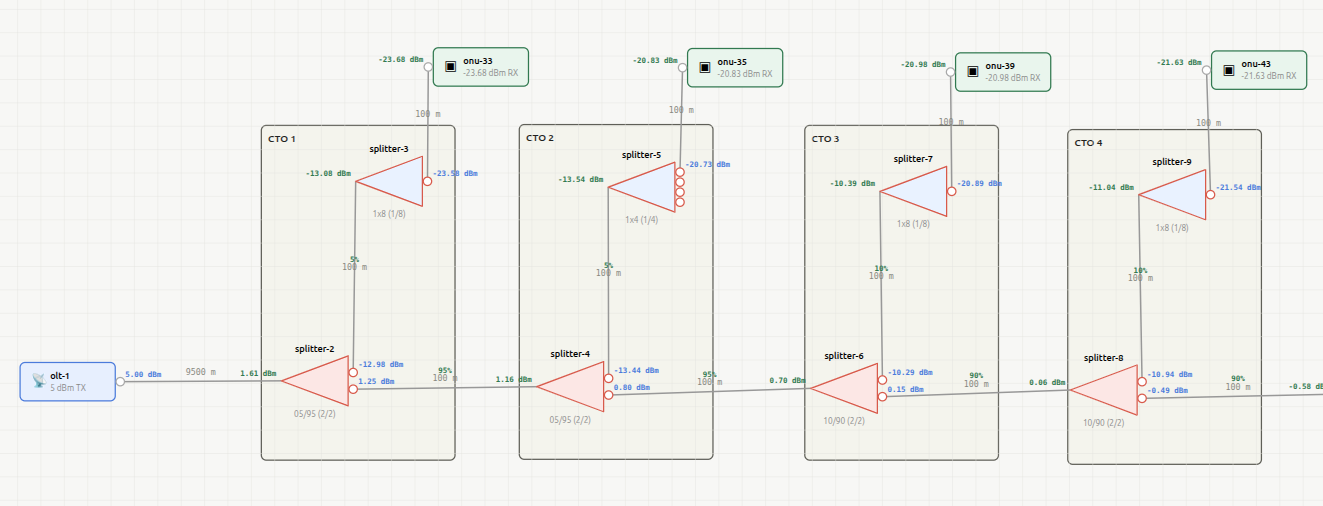
\includegraphics[width=0.95\textwidth]{images/ponplanner_ibirama_bal_bloco1.png}
        \par\footnotesize Fonte: Tela capturada da aplicação \textit{PON Planner}.
    }
\end{figure}

\begin{figure}[htb]
    \caption{Bloco 2 (Intermediário) da topologia balanceada no \textit{PON Planner} -- CTOs 06 a 10}
    \label{fig:ap_bal_b2}
    \centering
    \parbox{16cm}{
        \centering
        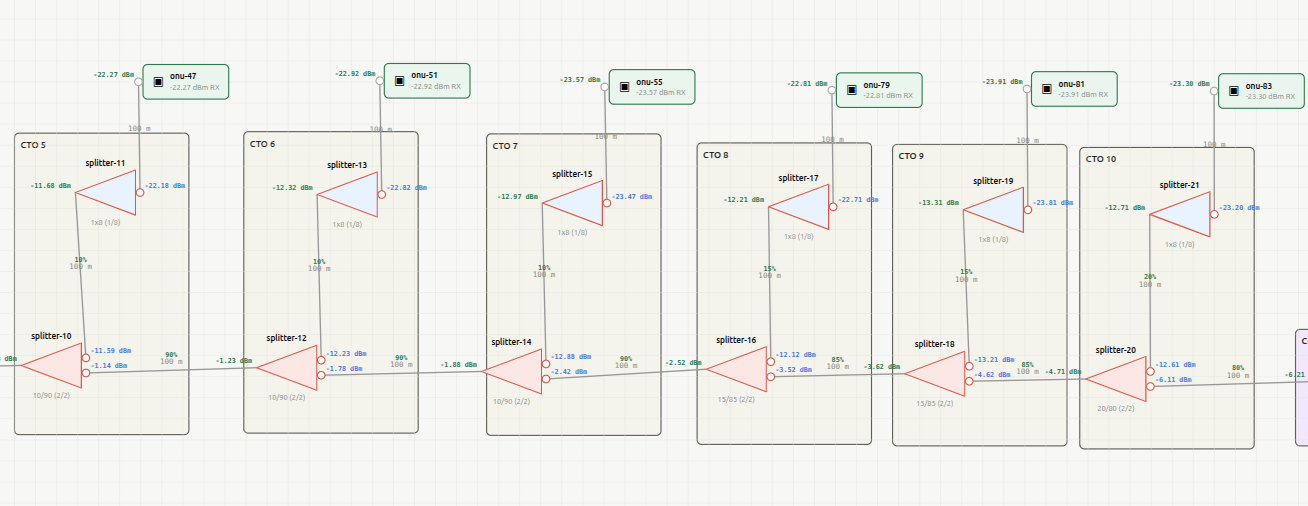
\includegraphics[width=0.95\textwidth]{images/ponplanner_ibirama_bal_bloco2.png}
        \par\footnotesize Fonte: Tela capturada da aplicação \textit{PON Planner}.
    }
\end{figure}

\begin{figure}[htb]
    \caption{Bloco 3 (Final) da topologia balanceada no \textit{PON Planner} -- CTOs 11 a 14 equalizadas}
    \label{fig:ap_bal_b3}
    \centering
    \parbox{16cm}{
        \centering
        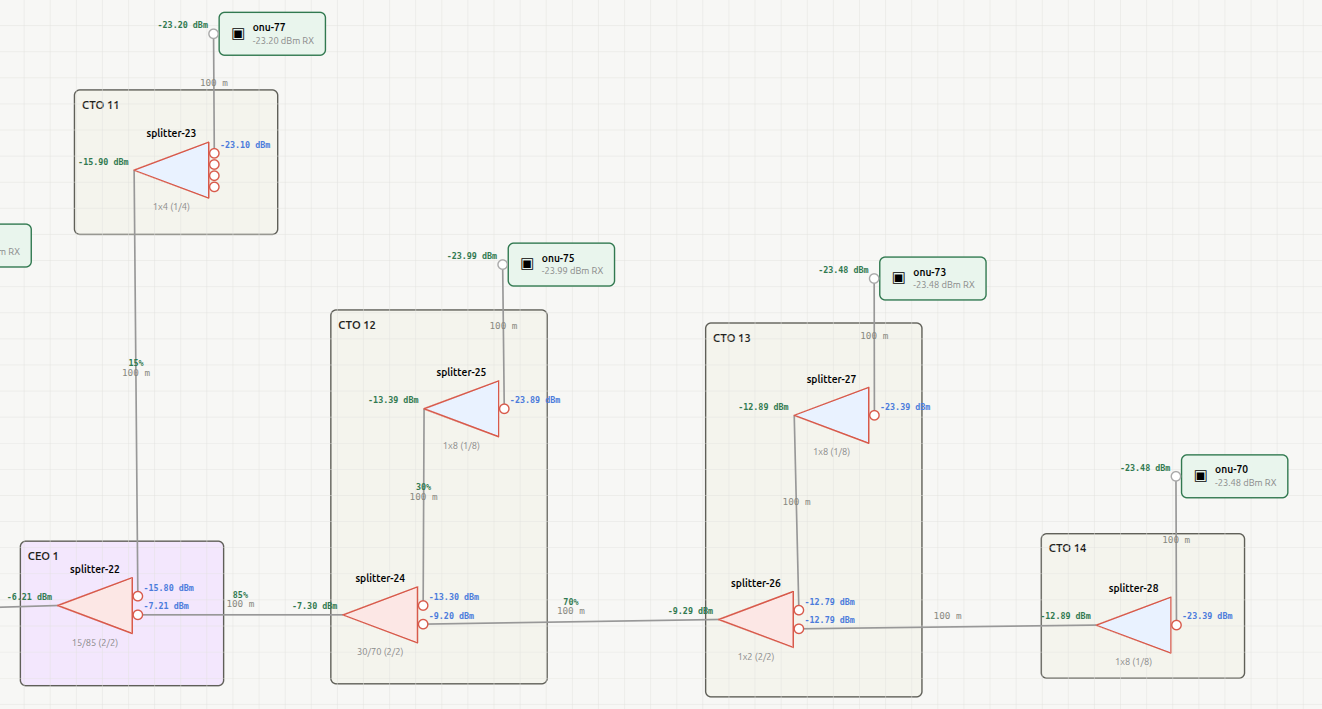
\includegraphics[width=0.95\textwidth]{images/ponplanner_ibirama_bal_bloco3.png}
        \par\footnotesize Fonte: Tela capturada da aplicação \textit{PON Planner}.
    }
\end{figure}

\end{apendicesenv}